\section{Sensor Quality Assessment}
\label{sec:QA}

\subsection{Full-Wafer Leakage Current}
\label{subsec:QA_Itot}

\begin{figure}
	\captionsetup[subfigure]{aboveskip=-1pt,belowskip=-1pt}
	\centering
	\begin{subfigure}[b]{0.49\textwidth}
		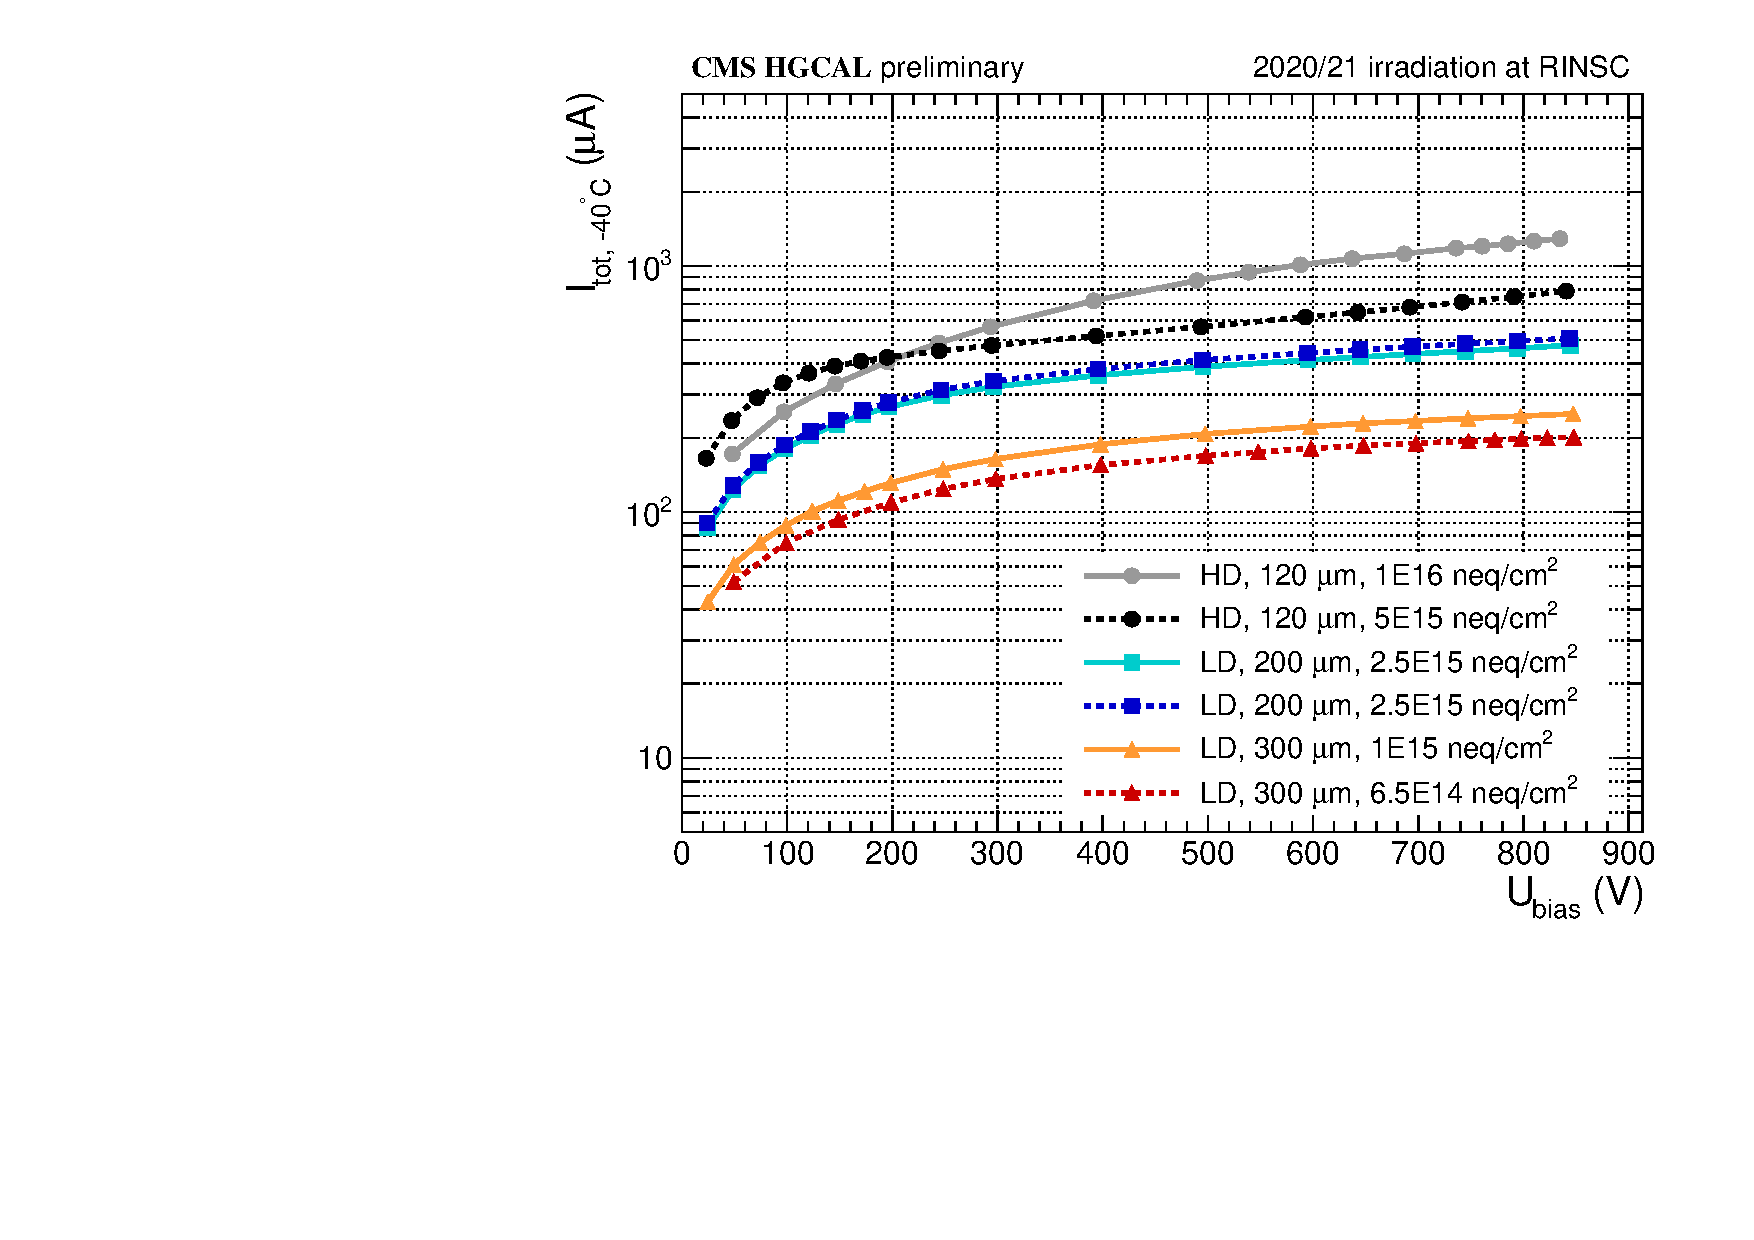
\includegraphics[width=0.999\textwidth]{plots/total_iv/total_current_IV.pdf}
		\subcaption{
		}
		\label{plot:tot_IV_good}
	\end{subfigure}
	\hfill
	\begin{subfigure}[b]{0.49\textwidth}
		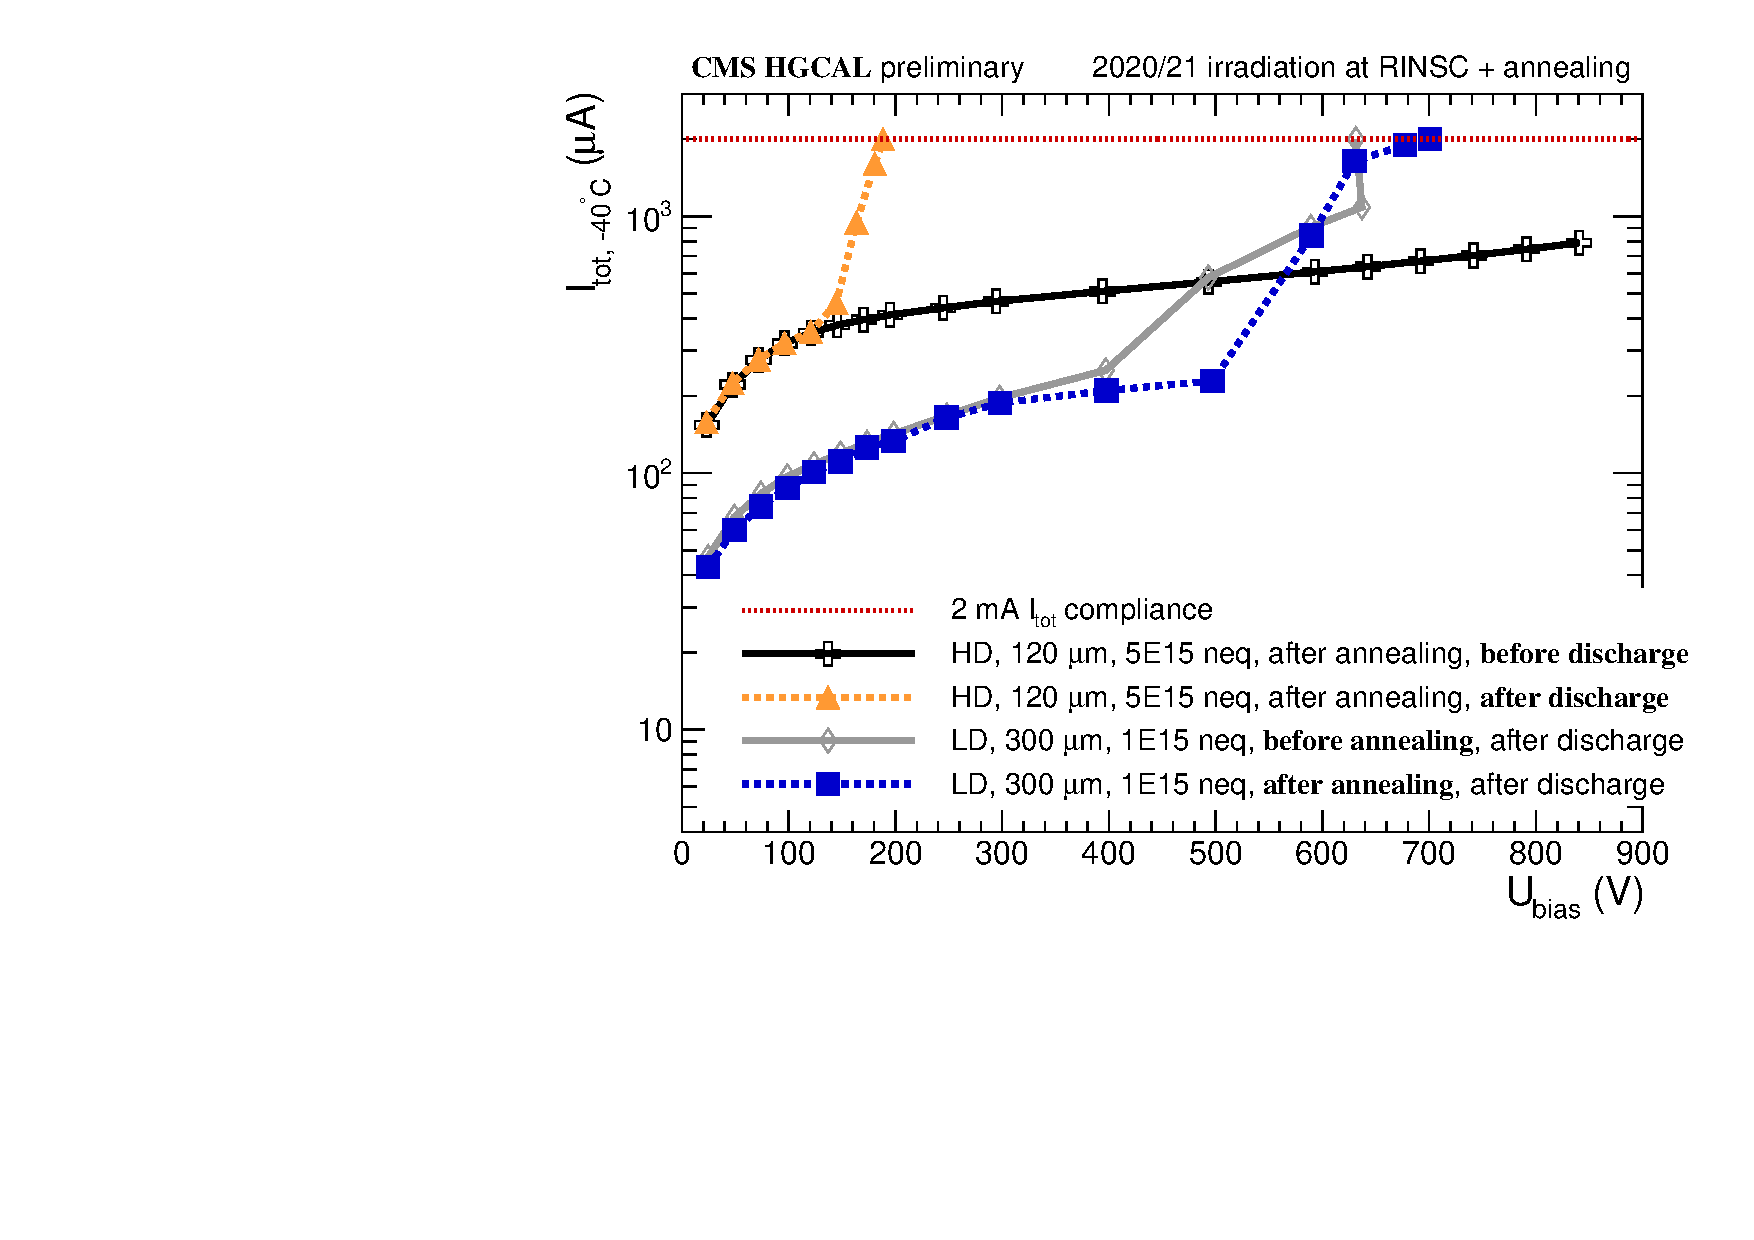
\includegraphics[width=0.999\textwidth]{plots/total_iv/total_current_IV_bad.pdf}
		\subcaption{
		}
		\label{plot:tot_IV_bad}
	\end{subfigure}
	\caption{
		(a) Full-wafer leakage currents at different effective bias voltages (a) for six good sensors from all irradiation rounds, and (b) for bad sensors with sudden leakage current increase.
	}
\end{figure}


\subsection{Per-Pad Leakage Currents}
\label{subsec:QA_Ipad}
\begin{figure}
	\captionsetup[subfigure]{aboveskip=-1pt,belowskip=-1pt}
	\centering
	\begin{subfigure}[b]{0.32\textwidth}
		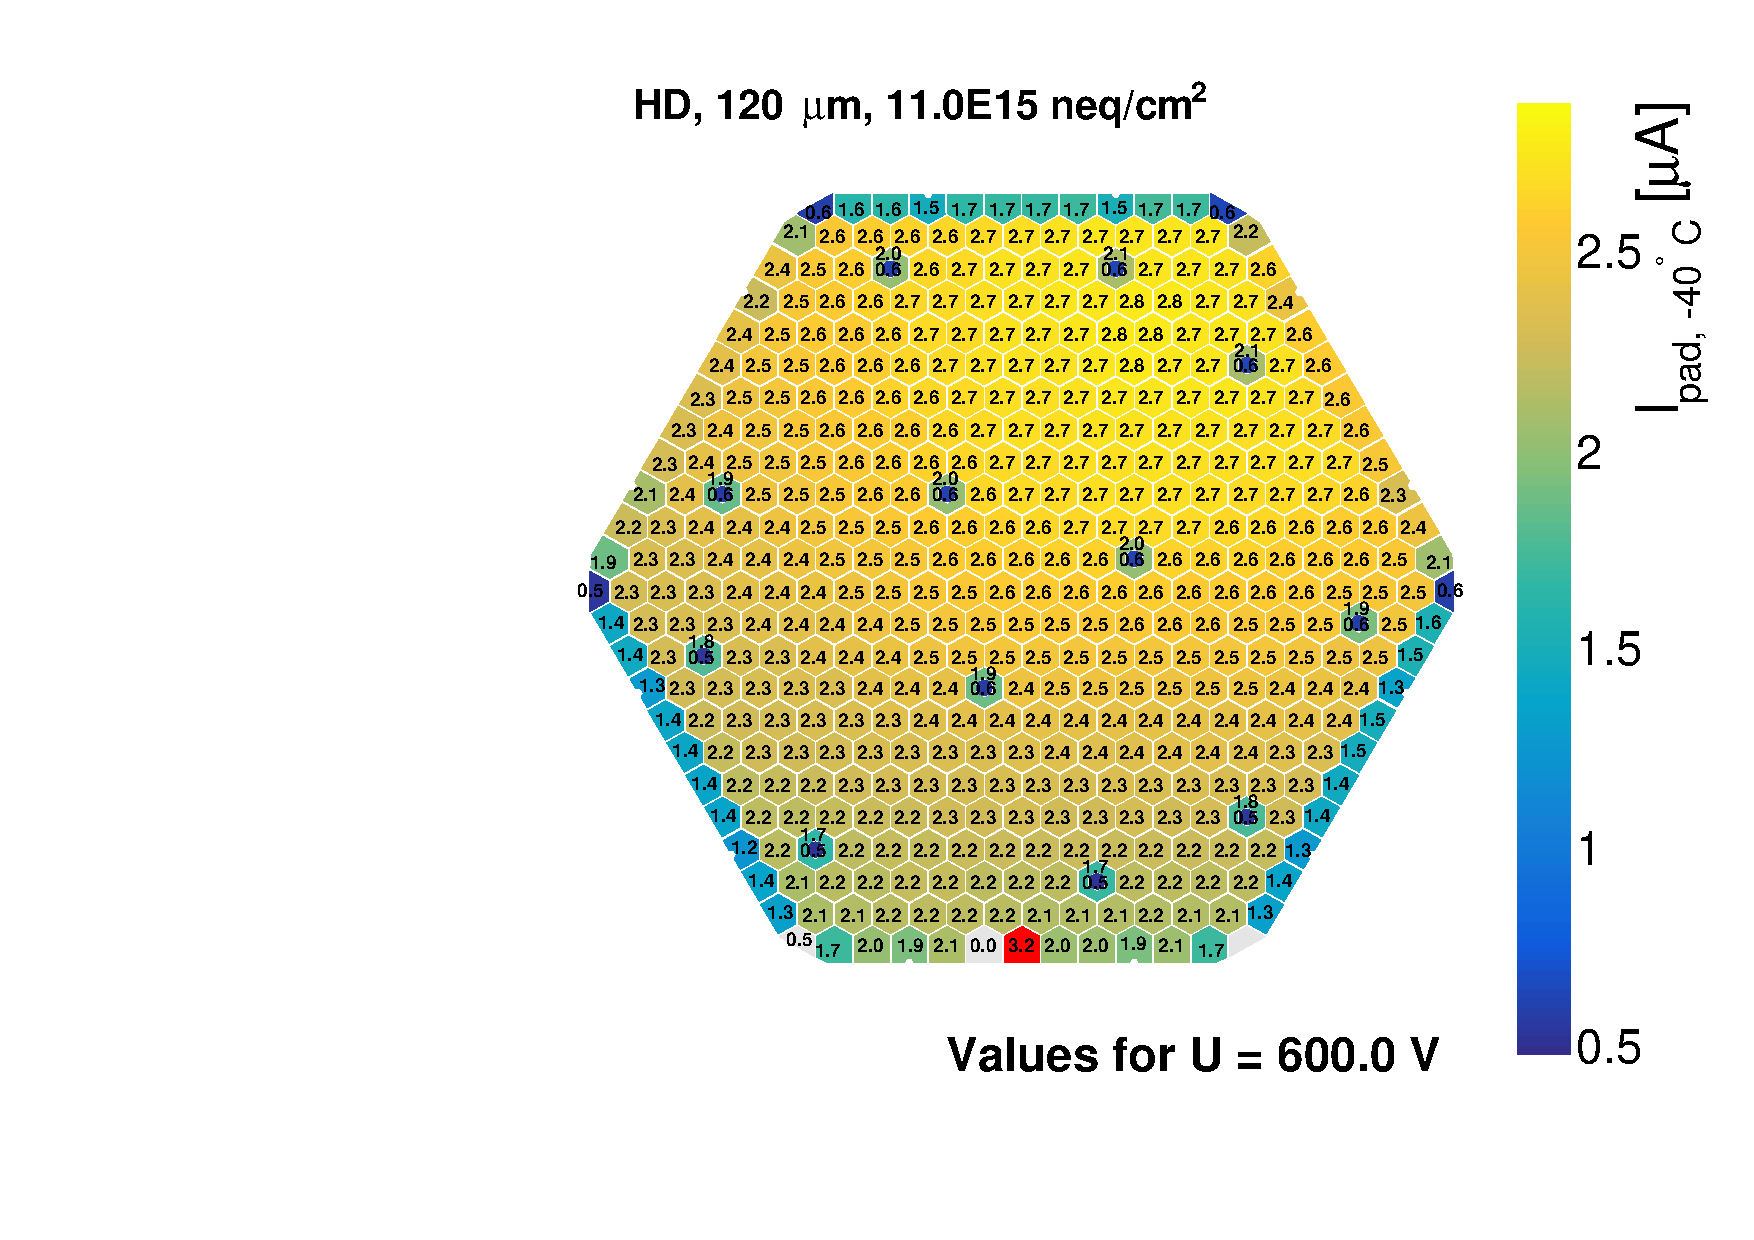
\includegraphics[width=0.999\textwidth]{plots/iv_hexplots/3003.pdf}
		\subcaption{
		}
		\label{plot:iv_hexplot_3003}
	\end{subfigure}
	\hfill
	\begin{subfigure}[b]{0.32\textwidth}
		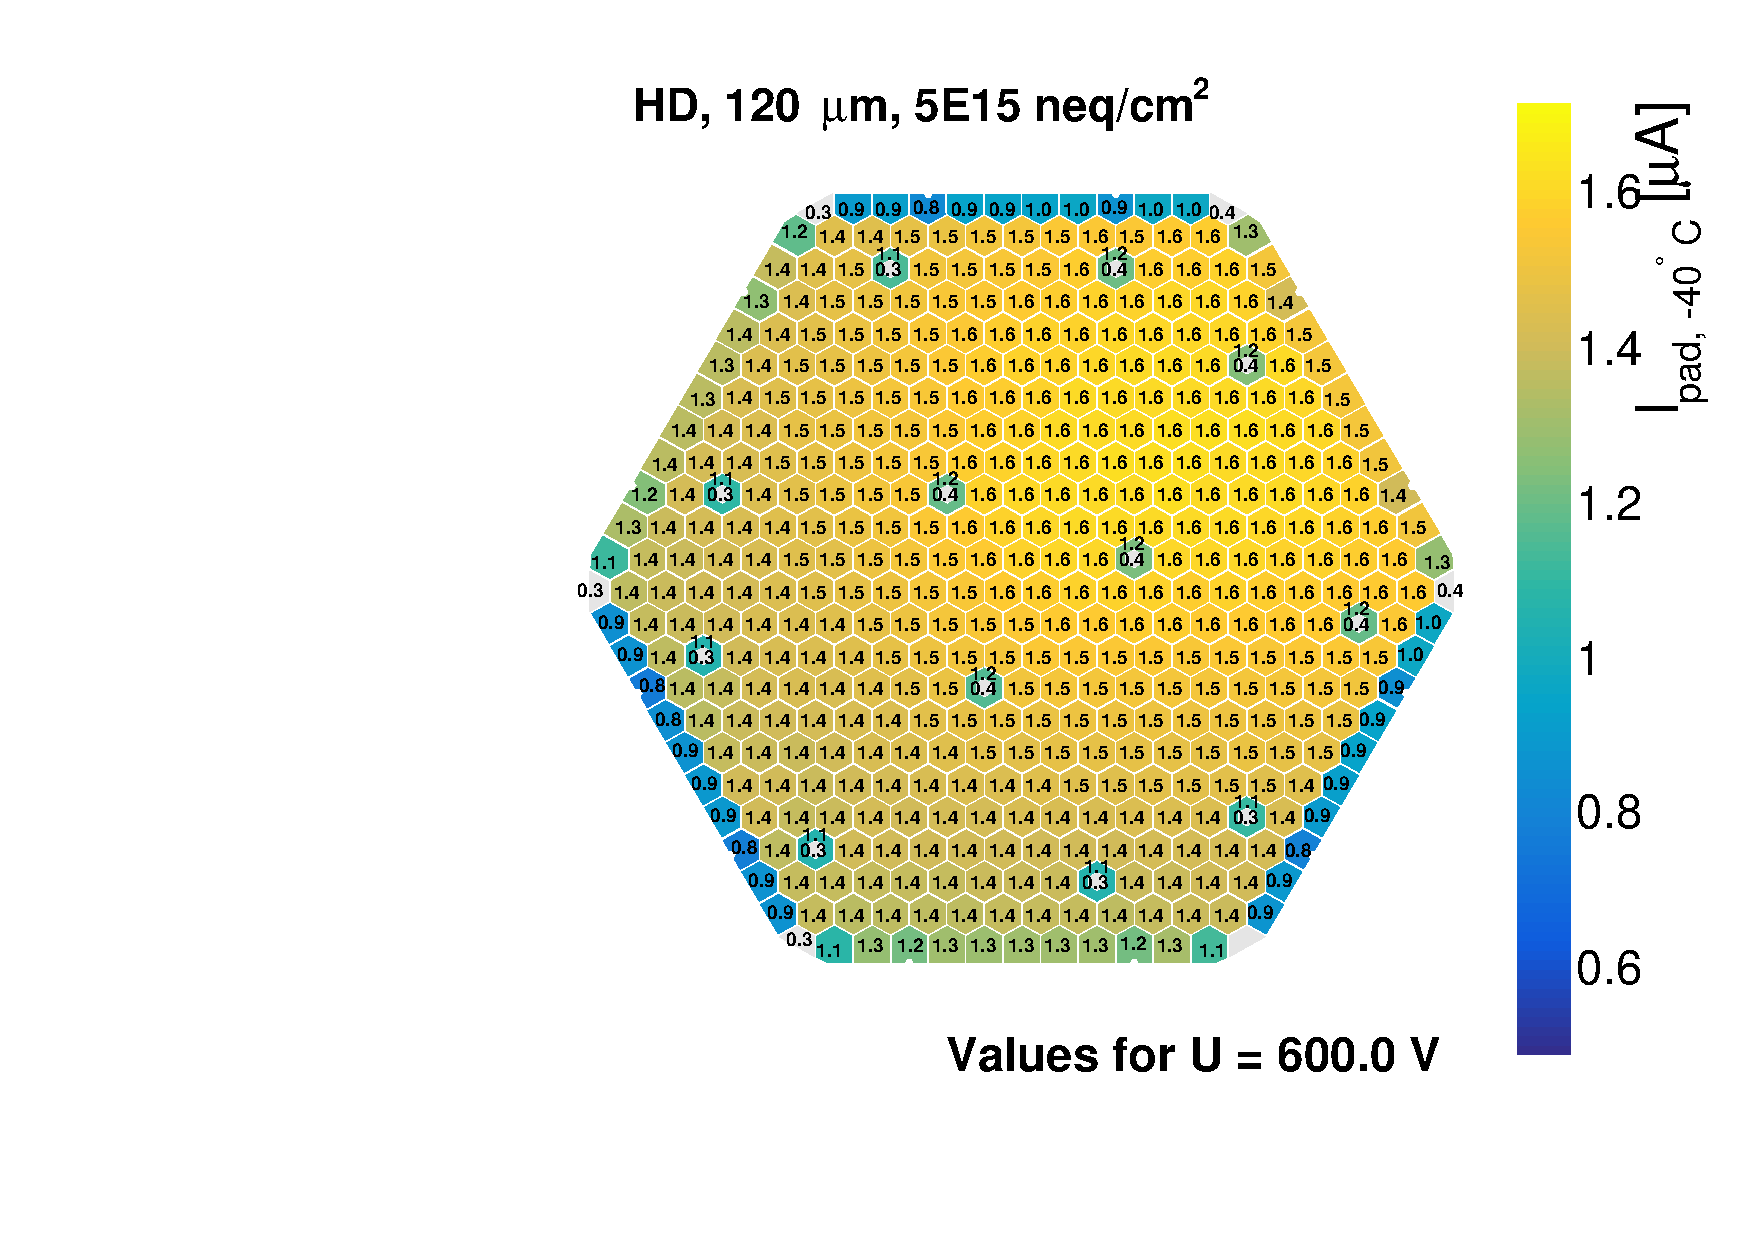
\includegraphics[width=0.999\textwidth]{plots/iv_hexplots/3009.pdf}
		\subcaption{
		}
		\label{plot:iv_hexplot_3009}
	\end{subfigure}
	\hfill
	\begin{subfigure}[b]{0.32\textwidth}
		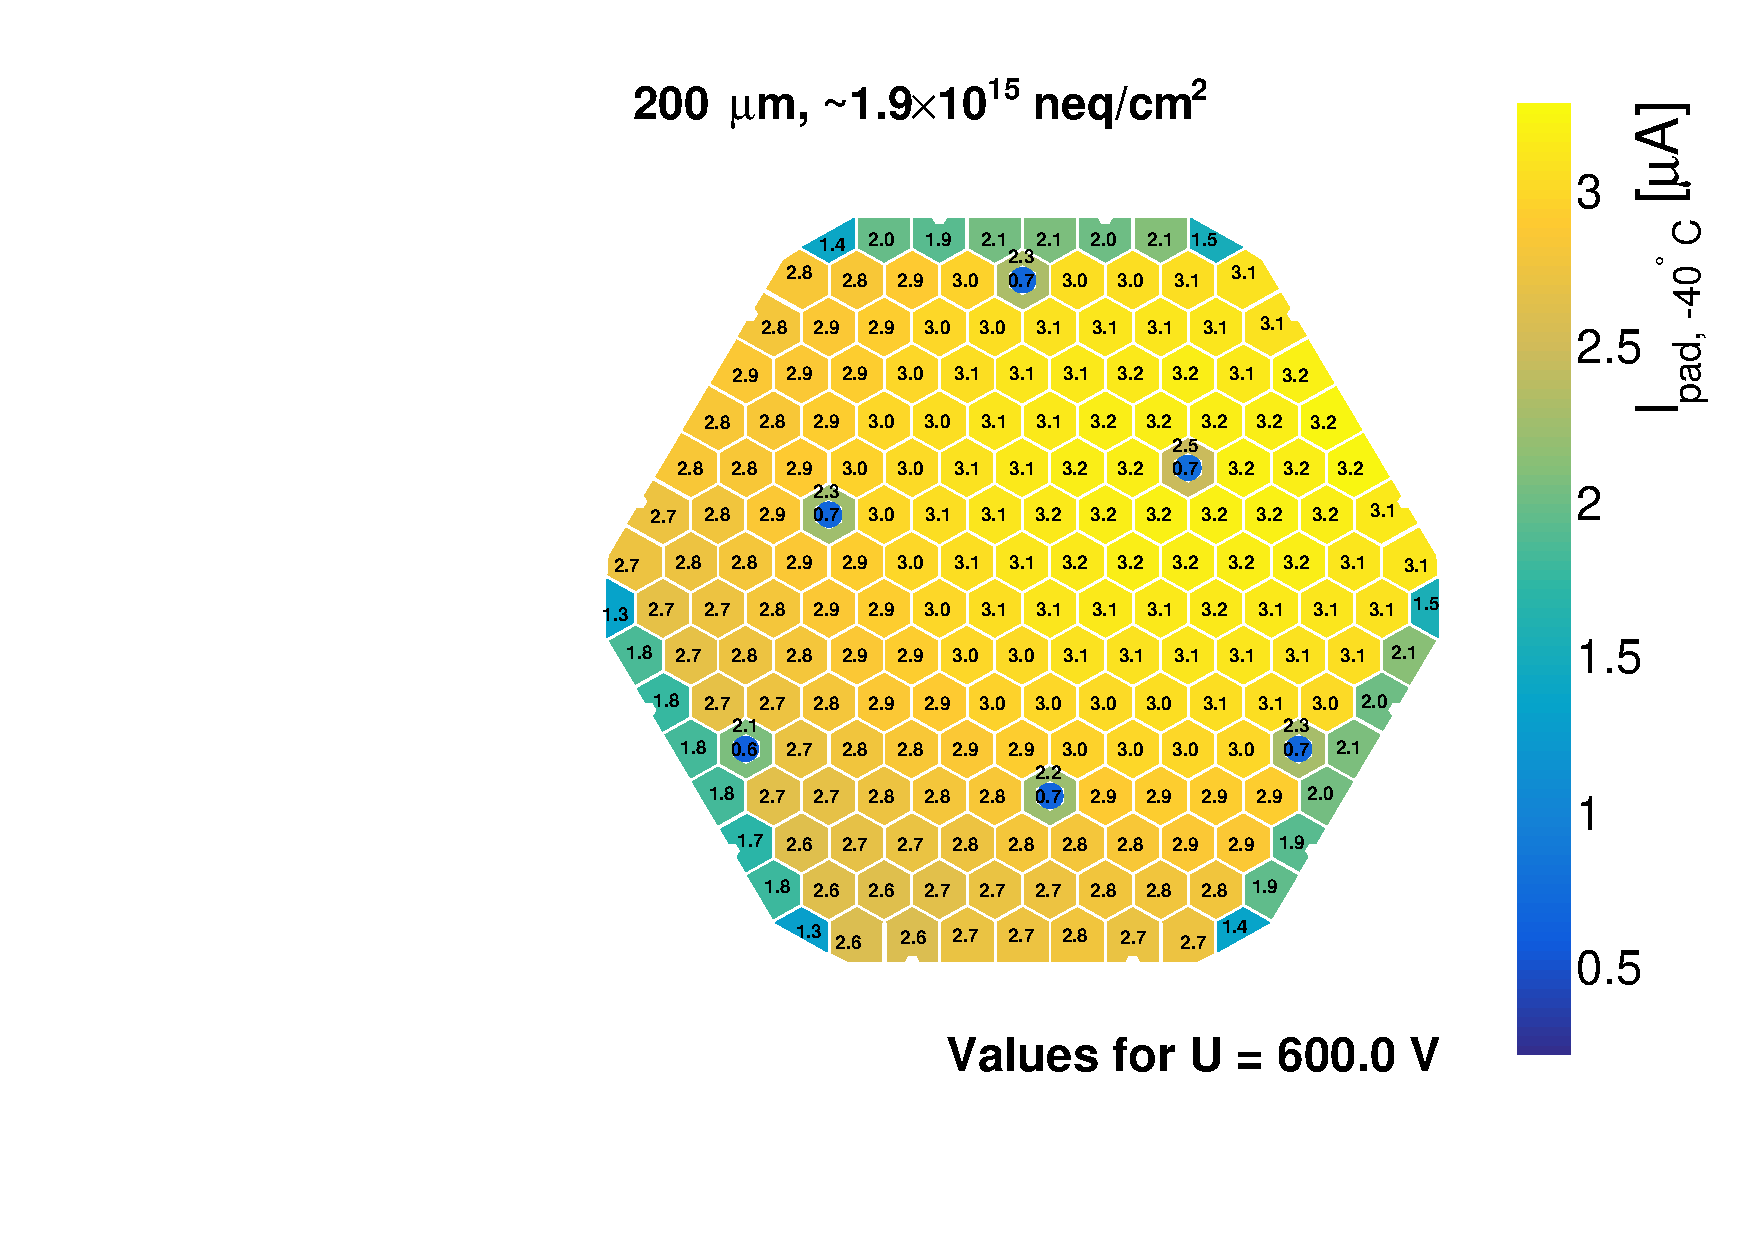
\includegraphics[width=0.999\textwidth]{plots/iv_hexplots/0541_04.pdf}
		\subcaption{
		}
		\label{plot:iv_hexplot_0541_04}
	\end{subfigure}
	\hfill	
	\begin{subfigure}[b]{0.32\textwidth}
		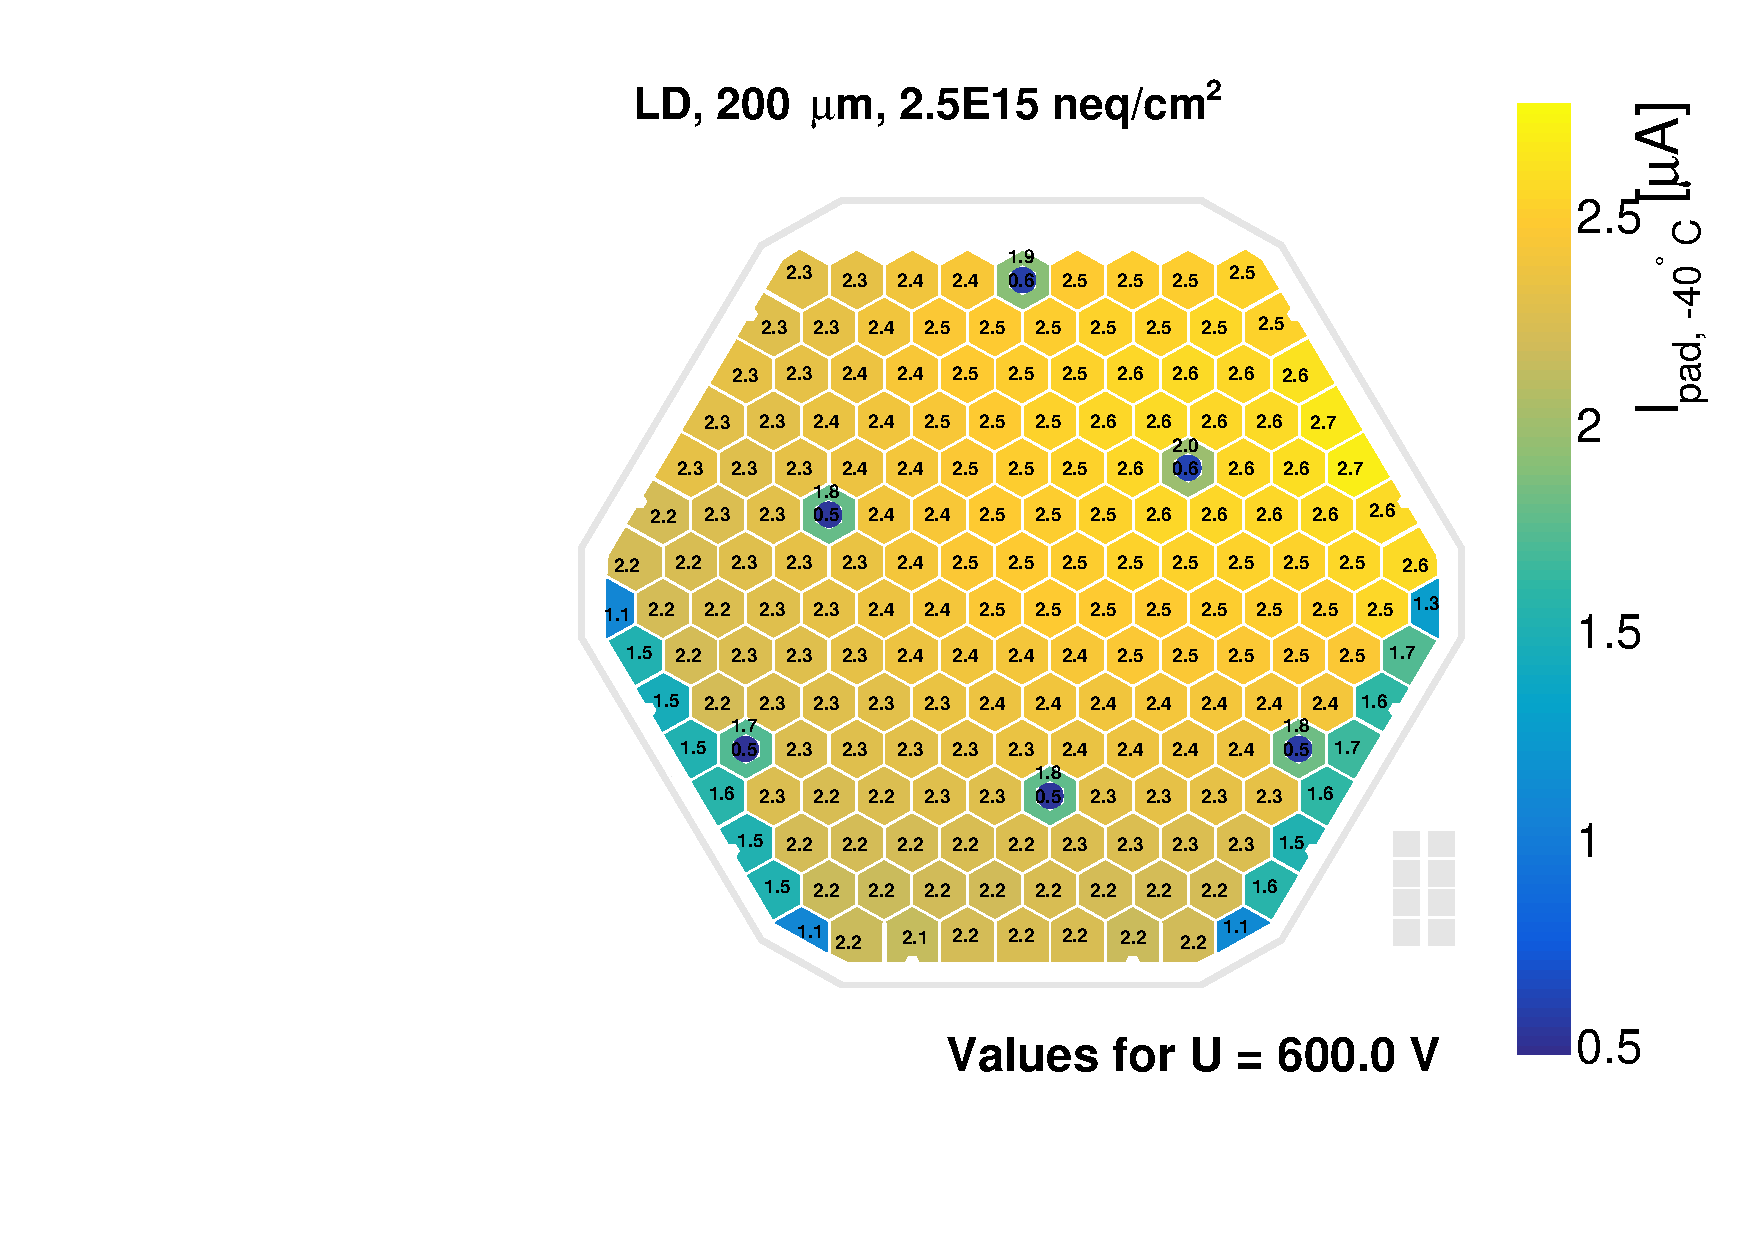
\includegraphics[width=0.999\textwidth]{plots/iv_hexplots/2004.pdf}
		\subcaption{
		}
		\label{plot:iv_hexplot_2004}
	\end{subfigure}
	\hfill
	\begin{subfigure}[b]{0.32\textwidth}
		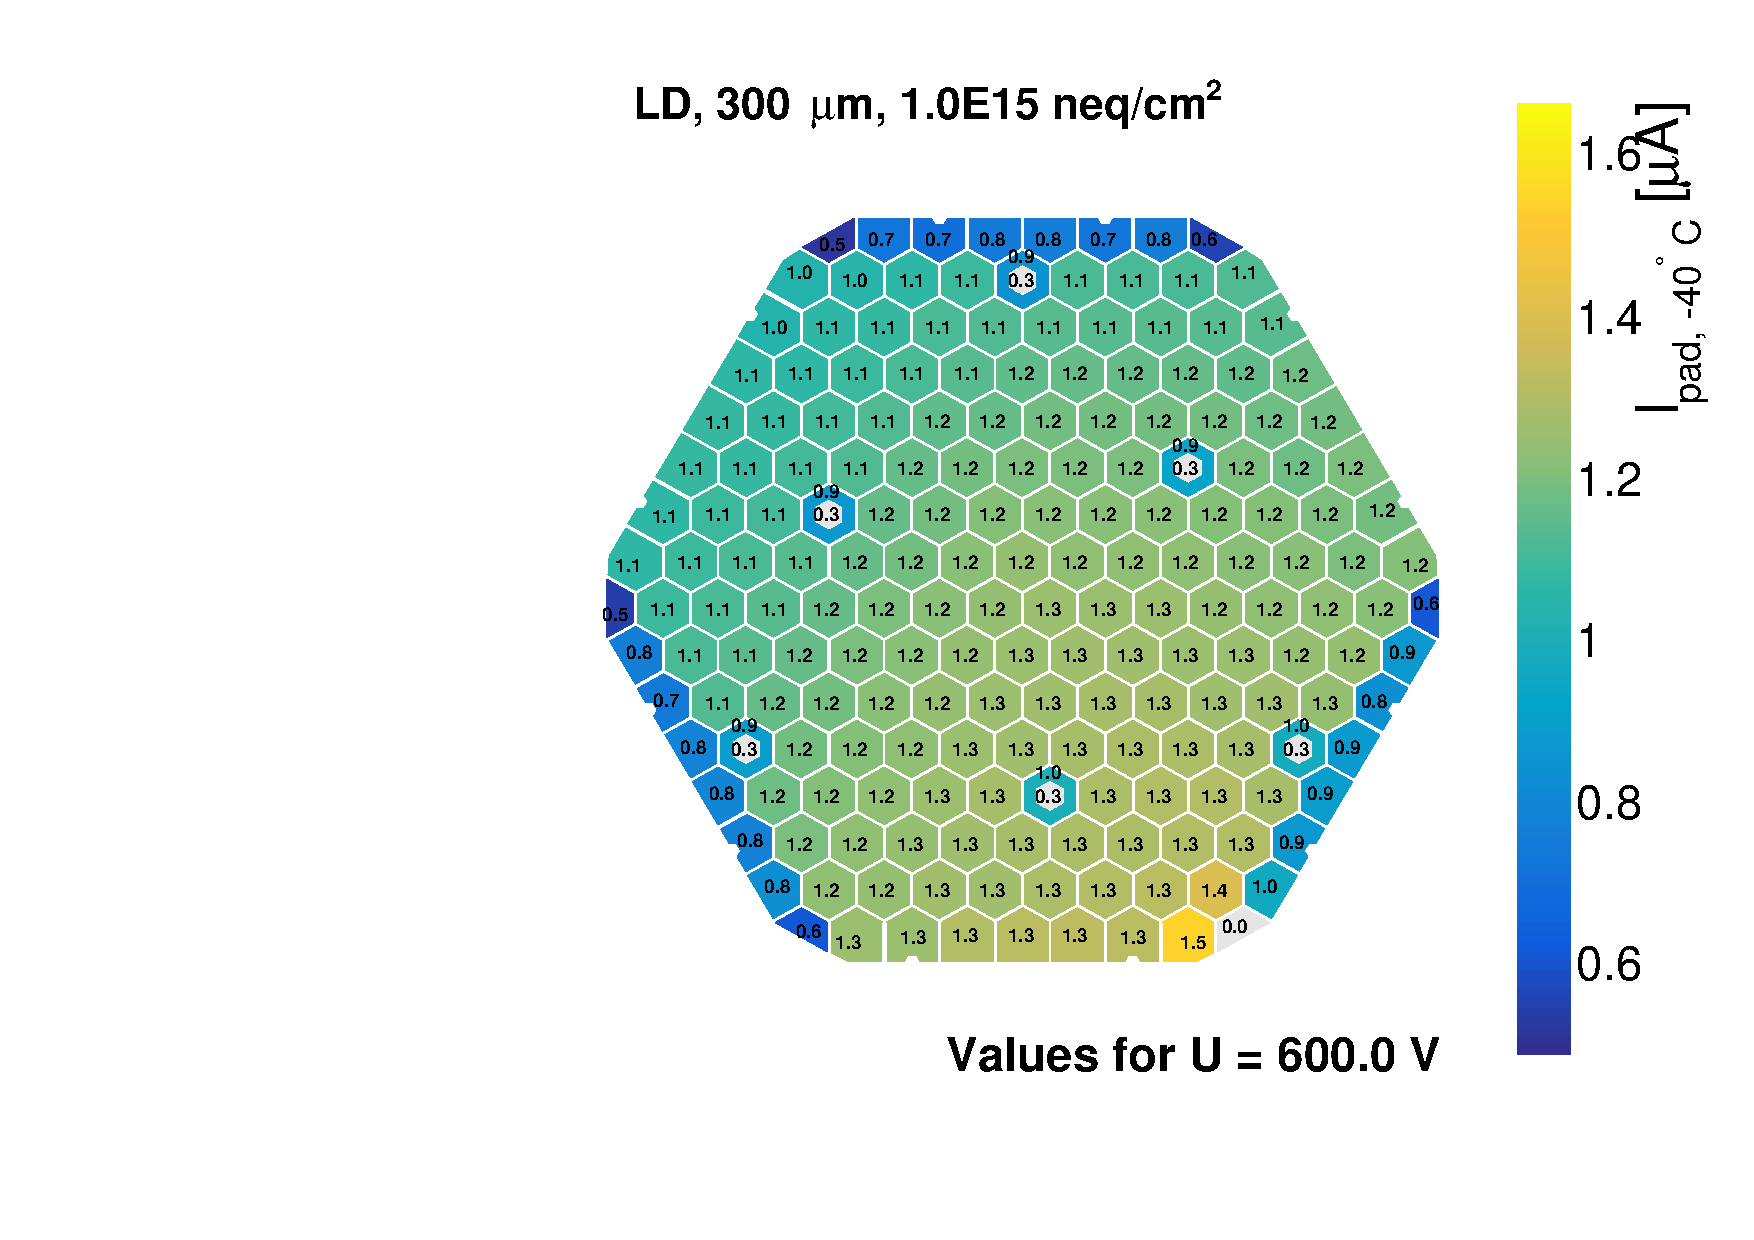
\includegraphics[width=0.999\textwidth]{plots/iv_hexplots/1013.pdf}
		\subcaption{
		}
		\label{plot:iv_hexplot_1013}
	\end{subfigure}
	\hfill
	\begin{subfigure}[b]{0.32\textwidth}
		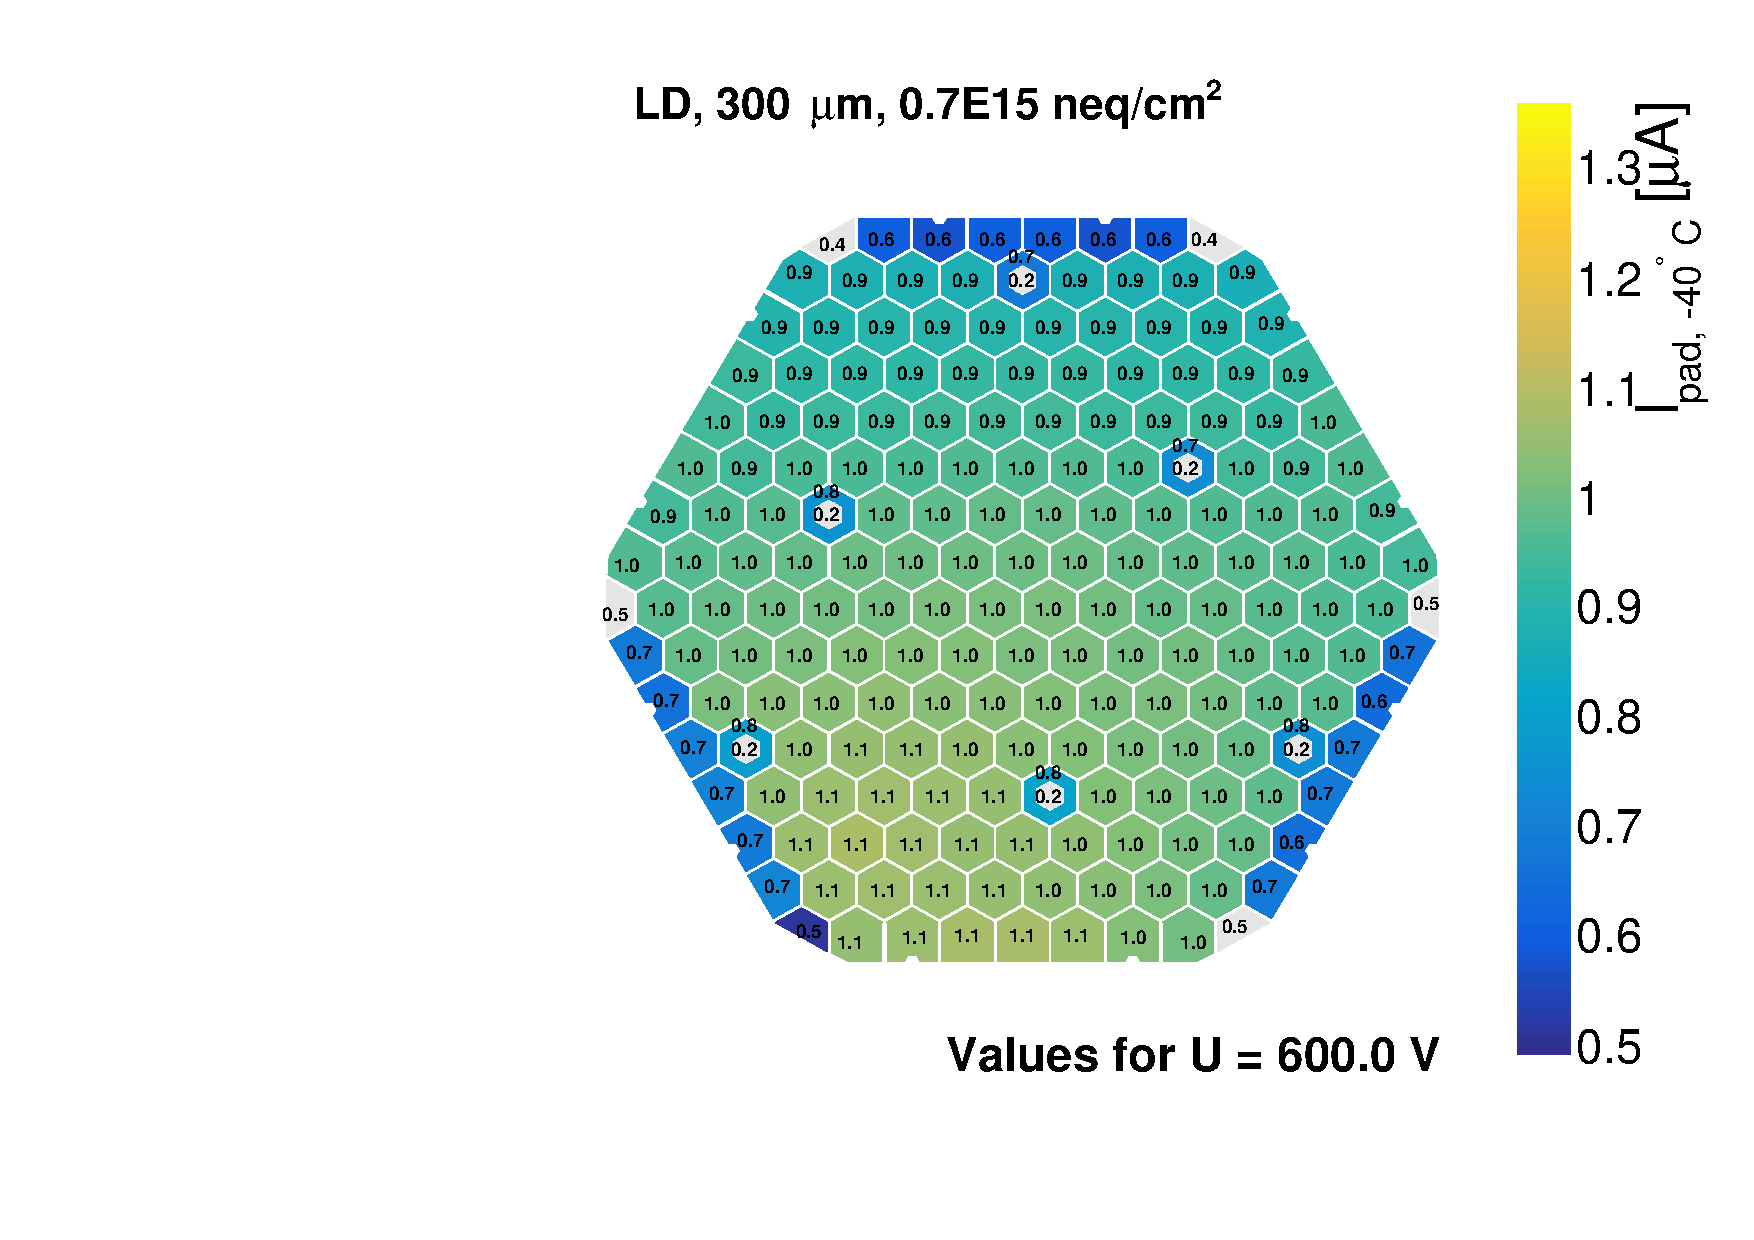
\includegraphics[width=0.999\textwidth]{plots/iv_hexplots/1002.pdf}
		\subcaption{
		}
		\label{plot:iv_hexplot_1002}
	\end{subfigure}	
	\caption{
		Per-pad leakage currents interpolated to an effective bias voltage of \SI{600}{\volt} for six representative sensors from all irradiation rounds.
		The chuck temperature profile is corrected for, cf.~\ref{appendix:chuck_temp}.
		Note the different leakage current scales.
		Red- or white-colored edge pads correspond to well-understood (however undesired) measurement peculiarities, e.g. unconnected pogo pins.
	}
\end{figure}

\subsection{Per-Pad Capacitance and Depletion Voltage}
\label{subsec:QA_Vdep}
